\documentclass{article}
\usepackage{hyperref} % For clickable links

\usepackage{ragged2e} % For justified text alignment
\usepackage{longtable}
\usepackage{booktabs} % For better table lines
\setlength{\parindent}{0pt} % Remove paragraph indentation
\usepackage{booktabs}
% Language setting
% Replace `english' with e.g. `spanish' to change the document language
\usepackage[english]{babel}
\usepackage{float} % To use [H] placement
% Set page size and margins
% Replace `letterpaper' with `a4paper' for UK/EU standard size
\usepackage[letterpaper,top=2cm,bottom=2cm,left=3cm,right=3cm,marginparwidth=1.75cm]{geometry}

% Useful packages
\usepackage{amsmath}
\usepackage{graphicx}

\usepackage{adjustbox} % To handle long rows
% \usepackage[colorlinks=true, allcolors=blue]{hyperref}

\onecolumn
\title{A Regression model to predict heat and cooling loads}
\author{Alberto Arath Figueroa Salomon}
\begin{document}

\maketitle

\section{Introduction}

Housing energy requirements are becoming increasingly demanding, as we switch 
from mechanical interfaces to digital ones, new electric car power demands.
Once crucial aspect of energy consumption are heat and cooling loads which can 
take up 50 percent of the power intake.

This model looks to find the features that make a house more energy efficency
as cooling and heat loads depend on the thermal capacity of the homes

\section{Data}

\subsection{Instance composition}
Data set is composed by labeled data, 707 rows and 64 features.
Training data has a synthetic origin so there is really no need for data preparation
which is good as we can focus solely in the application of Machine Learning techniques

% Table environment

\subsection{Predictor Set}

\begin{itemize}
    \item \( x_1 \): \textbf{Relative Compactness (RC)} Relative Compactness is a measure of how compact the building is. It can be represented as:
    \[
    RC = \frac{\text{Volume of the building}}{\text{Minimum envelope surface area for that volume}}
    \]

    \item \( x_2 \): \textbf{Surface Area (SA)} The total surface area of the building:
    \[
    SA = \text{Total Area of all external surfaces (walls, roof, floor, etc.)}
    \]

    \item \( x_3 \): \textbf{Wall Area (WA)} The area covered by the building's walls:
    \[
    WA = \text{Height of the wall} \times \text{Width of the wall}
    \]

    \item \( x_4 \): \textbf{Roof Area (RA)} The area covered by the building's roof:
    \[
    RA = \text{Length of the roof} \times \text{Width of the roof}
    \]

    \item \( x_5 \): \textbf{Overall Height (H)} The total height of the building:
    \[
    H = \text{Base to Top Height of the building}
    \]

    \item \( X_6 \): \textbf{Orientation (O)} Orientation describes the direction the building faces:
    \[
    O \in \{\text{North, South, East, West}\}
    \]

    \item \( X_7 \): \textbf{Glazing Area (GA)} The total area of walls that are made of glass:
    \[
    GA = \text{Sum of all glassed surfaces (windows, panels, etc.)}
    \]

    \item \( X_8 \): \textbf{Glazing Area Distribution (GAD)}\\
    The distribution of glazing area across the building:
    \[
    GAD = \frac{\text{Glazing Area in a particular wall}}{\text{Total Glazing Area}}
    \]
   
\end{itemize}
\subsection{Categorical Variable Handling}
\textbf{Orientation (O)} Is categorical variable, One Hot Encoder column insetion
is being used to treat this feature into the model

\subsection{Target Variables}
\begin{itemize}
    \item \( y_1 \): \textbf{Heating Load (HL)}\\
    The total load required to heat the building, expressed as:
    \[
    HL = f(X_1, X_2, X_3, X_4, X_5, X_6, X_7, X_8)
    \]
    
    \item \( y_2 \): \textbf{Cooling Load (CL)}\\
    The total load required to cool the building, expressed as:
    \[
    CL = f(X_1, X_2, X_3, X_4, X_5, X_6, X_7, X_8)
    \]
\end{itemize}
This encoding To allows the application of machine learning algorithms such as softmax regression, decision trees, or neural networks to predict the likelihood of each class based on the input features.

\section{Exploratory Data Analysis (EDA)}

\subsection{Correlation Matrix}

Feature set shows a strong correlation in clusters
a PCA aproach might work help even though there aren't that many features.

\begin{figure}[H]  
    \centering
    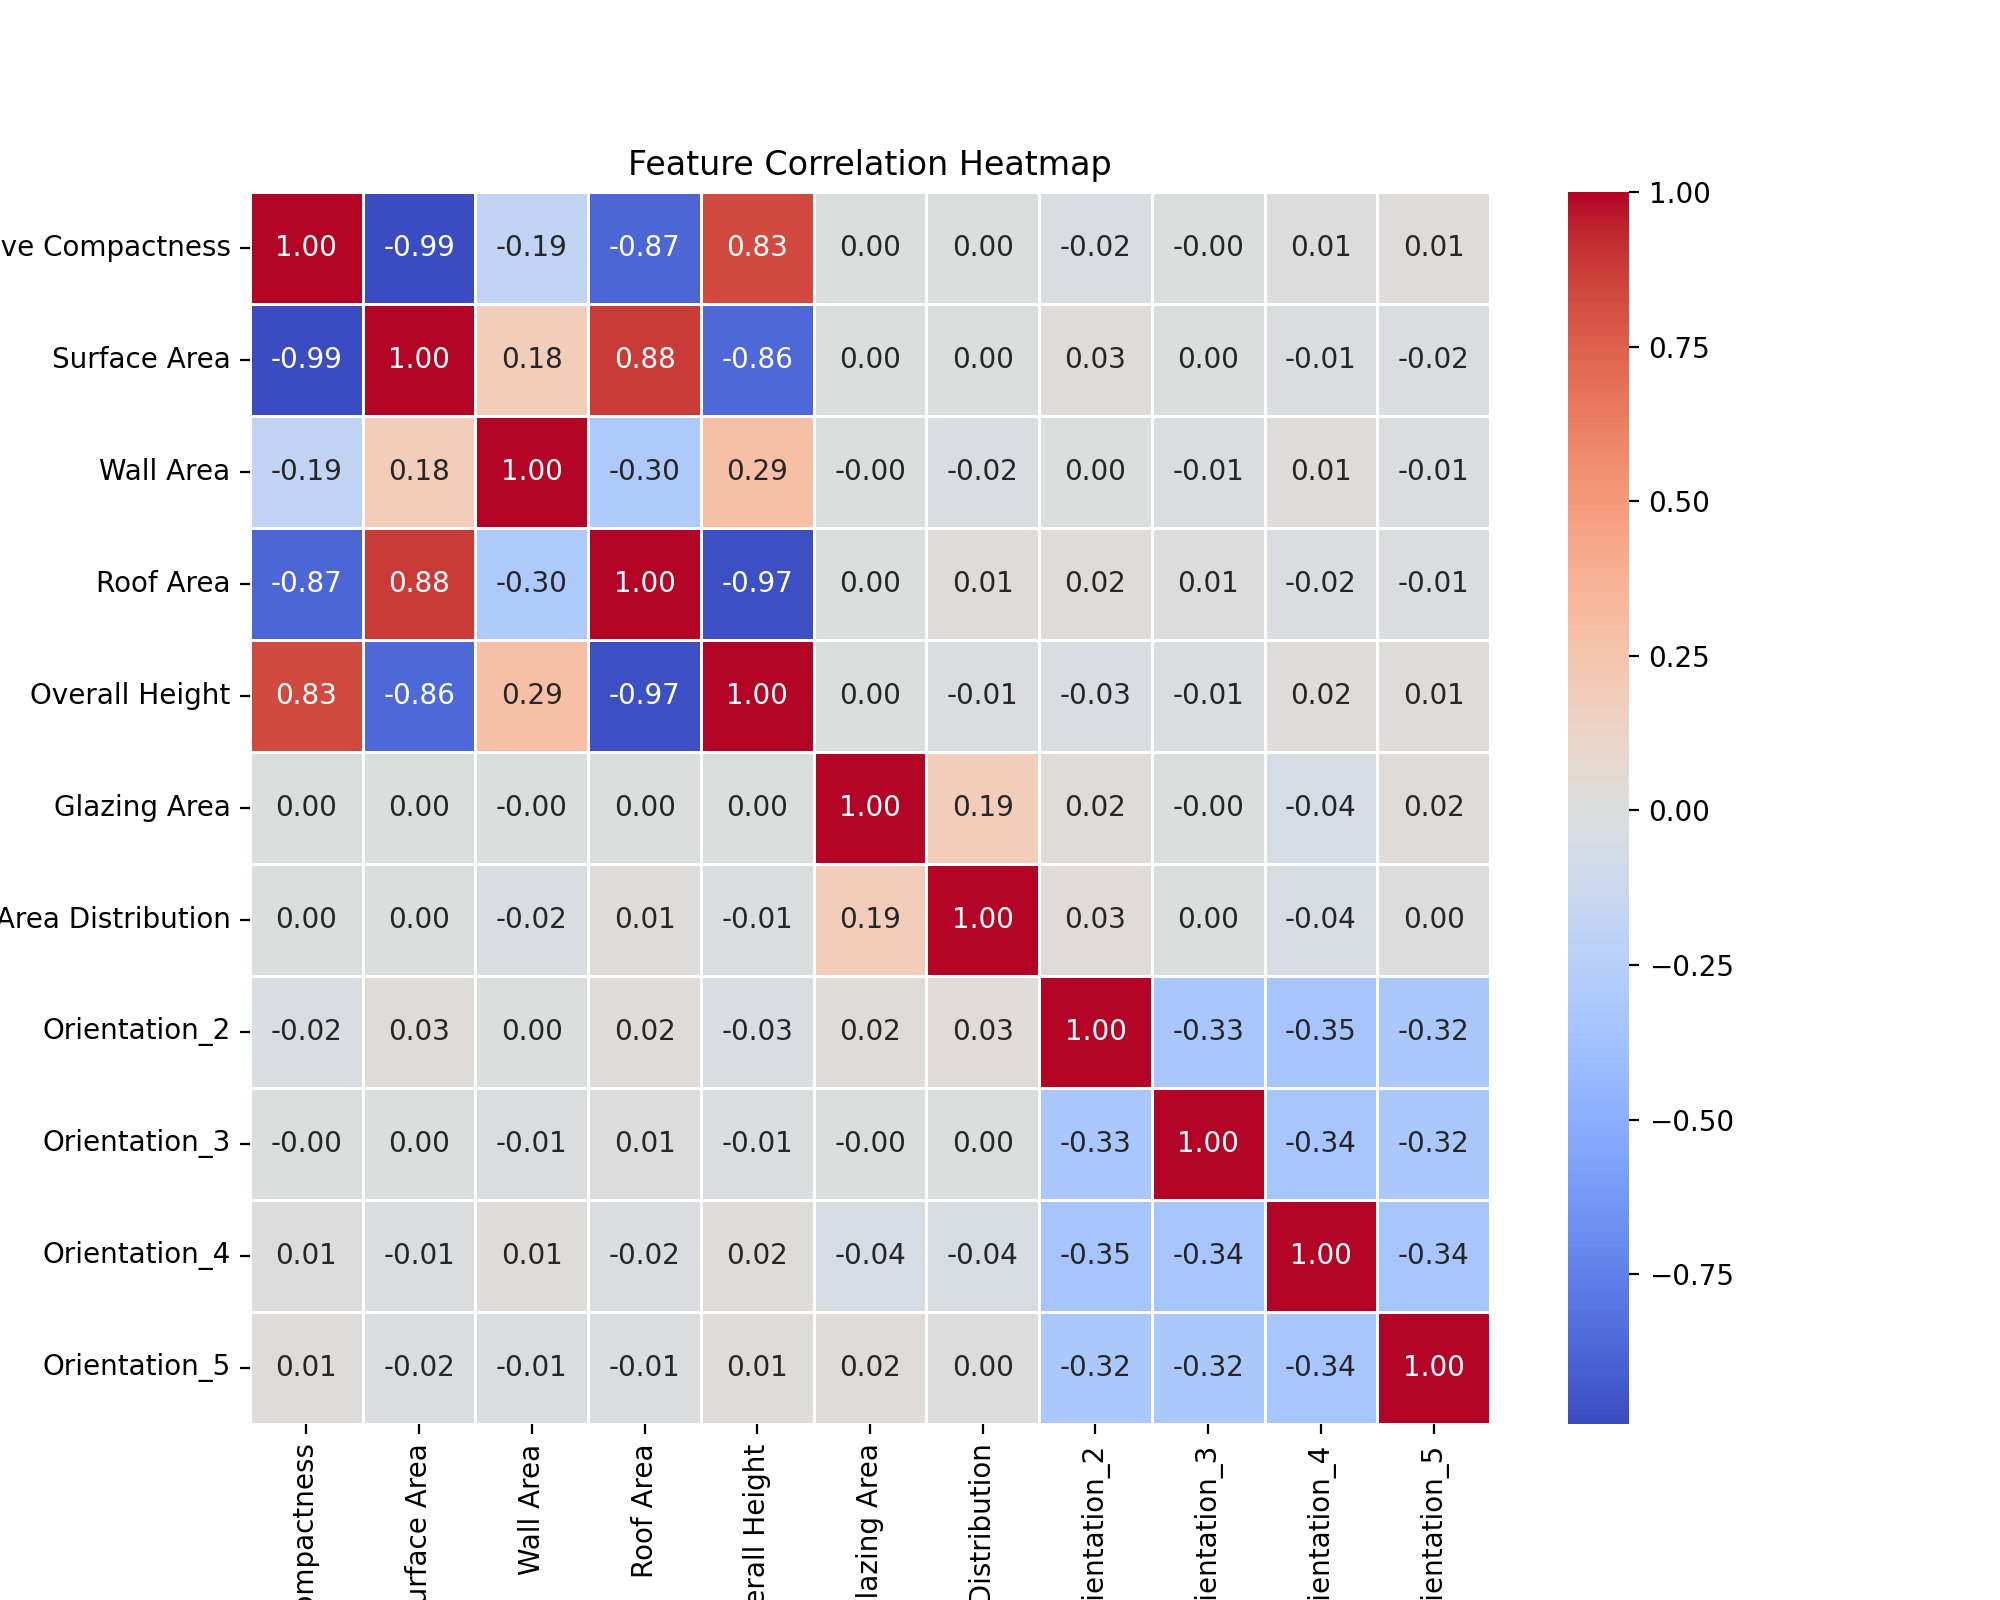
\includegraphics[width=1\linewidth]{Feature_Correlation_Heatmap.png}
    \caption{Features Correlation Heat marginparwidth}
    \vspace{-1em} % Reduce vertical spacing
    \end{figure}

\subsection{Features correaltion matrix}


\section{Methodology}
In this study, we performed hyperparameter tuning using Grid Search, testing multiple machine learning algorithms to identify the best-performing model. The following algorithms were evaluated:

\subsection{Metric used}

\subsection*{Root Mean Squared Error (RMSE)}

The RMSE measures the square root of the average squared differences between predicted and actual values. It is given by:

\[
\text{RMSE} = \sqrt{\frac{1}{n} \sum_{i=1}^n (y_i - \hat{y}_i)^2}
\]

Where:
\begin{itemize}
    \item \( y_i \): Actual value,
    \item \( \hat{y}_i \): Predicted value,
    \item \( n \): Number of samples.
\end{itemize}

\subsection*{R-Squared (R²)}

The R-Squared score measures the proportion of variance explained by the model. It is defined as:

\[
R^2 = 1 - \frac{\sum_{i=1}^n (y_i - \hat{y}_i)^2}{\sum_{i=1}^n (y_i - \bar{y})^2}
\]

Where:
\begin{itemize}
    \item \( y_i \): Actual value,
    \item \( \hat{y}_i \): Predicted value,
    \item \( \bar{y} \): Mean of actual values,
    \item \( n \): Number of samples.
\end{itemize}

\subsection{Pre-processing algorithms}

\begin{itemize}
    \item \textbf{Standard Feature Regularization:} \\
    Standardizes features by centering them at zero and scaling to unit variance:
    \[
    z = \frac{x - \mu}{\sigma}
    \]
    Where:
    \begin{itemize}
        \item \( x \): Original feature value.
        \item \( \mu \): Mean of the feature.
        \item \( \sigma \): Standard deviation of the feature.
    \end{itemize}
    
    \item \textbf{One-Hot Encoding (OHE):} \\
    Converts a categorical variable into binary features, one for each class:
    \[
    \text{OHE}(x) = [x_1, x_2, \dots, x_k], \quad x_i \in \{0, 1\}, \quad \sum_{i=1}^k x_i = 1
    \]
    Where:
    \begin{itemize}
        \item \( k \): Number of unique classes.
        \item \( x_i \): Binary variable indicating presence (\( 1 \)) or absence (\( 0 \)) of class \( i \).
    \end{itemize}

    \item \textbf{Principal Component Analysis (PCA):} \\
    PCA reduces dimensionality by transforming data into a new set of axes (principal components). The optimal number of components (axes) can be found iteratively using Grid Search with Cross-Validation (2-folds):
    \begin{itemize}
        \item Each fold evaluates the cross-validation score.
        \item Grid Search determines the number of principal components that maximize the model's performance.
    \end{itemize}

\end{itemize}
\subsection{Linear Regression Model}
if there aren't regularization techniques and instance set is not too large,
solver will use will use normal equation if not specified. Normal equation is used to compute weights.


\subsection{Hyperparameter Tuning}
Grid search was used to determine best number of axis 
in PCA, this is more for the sake of study as no much improvement is expected
\begin{table}[h!]
    \centering
    \caption{Hyperparameter Combinations and Corresponding Test Scores with 2 k folds}
    \label{tab:hyperparam_scores}
    \begin{tabular}{lcc}
    \toprule
    \textbf{Hyperparameter Combination} & \textbf{Mean Test Score} & \textbf{Rank Test Score} \\
    \midrule
    Preprocessing num pipeline PCA components = 5 & 0.8945 & 1 \\
    Preprocessing num pipeline PCA components = 3 & 0.8384 & 2 \\
    Preprocessing num pipeline PCA components = 1 & 0.6438 & 3 \\
    \bottomrule
    \end{tabular}
    \end{table}


\section{Results and Discussion}

Results are not that exciting model performs reasonable well for a 95 percent variance
acceptance

\begin{table}[h!]
    \centering
    \caption{Training and Test Set Performance Metrics}
    \label{tab:performance_metrics}
    \renewcommand{\arraystretch}{1.2} % Adjust row spacing
    \begin{tabular}{lcc}
        \toprule
        \textbf{Metric} & \textbf{Training Set} & \textbf{Test Set} \\
        \midrule
        RMSE            & 3.0672               & 3.1580           \\
        \( R^2 \)       & 0.9481               & 0.9506           \\
        \bottomrule
    \end{tabular}
\end{table}

Scikit-learn has been widely used for machine learning tasks \cite{disease_dataset2023}. Vector-borne diseases are a significant challenge\cite{disease_dataset2023}.

\appendix
\section{Additional tables}


\label{sec:appendix}
\bibliographystyle{alpha}
\bibliography{references}
\end{document}